\documentclass{article}

\usepackage[utf8]{inputenc}
\usepackage[russian]{babel}
\usepackage[a4paper, margin=1in]{geometry}
\usepackage{graphicx}
\usepackage{amsmath}
\usepackage{wrapfig}
\usepackage{multirow}
\usepackage{mathtools}
\usepackage{pgfplots}
\usepackage{pgfplotstable}
\usepackage{setspace}
\usepackage{changepage}
\usepackage{caption}
\usepackage{csquotes}
\usepackage{hyperref}
\usepackage{listings}

\pgfplotsset{compat=1.18}
\hypersetup{
  colorlinks = true,
  linkcolor  = blue,
  filecolor  = magenta,      
  urlcolor   = darkgray,
  pdftitle   = {
    math-tool-report-approx-smirnov-victor-p32131
  },
}

\definecolor{codegreen}{rgb}{0,0.6,0}
\definecolor{codegray}{rgb}{0.5,0.5,0.5}
\definecolor{codepurple}{rgb}{0.58,0,0.82}
\definecolor{backcolour}{rgb}{0.99,0.99,0.99}

\lstdefinestyle{codestyle}{
  backgroundcolor=\color{backcolour},   
  commentstyle=\color{codegreen},
  keywordstyle=\color{magenta},
  numberstyle=\tiny\color{codegray},
  stringstyle=\color{codepurple},
  basicstyle=\ttfamily\footnotesize,
  breakatwhitespace=false,         
  breaklines=true,                 
  captionpos=b,                    
  keepspaces=true,                 
  numbers=left,                    
  numbersep=5pt,                  
  showspaces=false,                
  showstringspaces=false,
  showtabs=false,                  
  tabsize=2
}

\lstset{style=codestyle}

\begin{document}

\begin{titlepage}
    \begin{center}
        \begin{spacing}{1.4}
            \large{Университет ИТМО} \\
            \large{Факультет программной инженерии и компьютерной техники} \\
        \end{spacing}
        \vfill
        \textbf{
            \huge{Теория Вероятности.} \\
            \huge{Практическая работа №5.} \\
        }
    \end{center}
    \vfill
    \begin{center}
        \begin{tabular}{r l}
            Группа:  & P32131                  \\
            Студент: & Смирнов Виктор Игоревич \\
            Вариант: & 16                      \\
        \end{tabular}
    \end{center}
    \vfill
    \begin{center}
        \begin{large}
            2023
        \end{large}
    \end{center}
\end{titlepage}

\section{Исходный код}

\subsection{Модуль для вычисления основных статистических показателей}

\lstinputlisting[
    language={Python},
    caption={Модуль для вычисления основных статистических показателей},
]{./stati.py}

\subsection{Модуль для отрисовки графиков}

\lstinputlisting[
    language={Python},
    caption={Модуль для отрисовки графиков},
]{./ploti.py}

\subsection{Скрипт для обработки данных}

\lstinputlisting[
    language={Python},
    caption={Скрипт для обработки данных},
]{./lab5.py}

\section{Результаты работы программы}

\subsection{Вывод в терминал}

\begin{lstlisting}[
    language={Bash},
    caption={Результаты вывода программы}
]
$ python3 lab5.py
Probability Theory Assignment 1 by Smirnov Victor
Input data:
[-0.45, 0.52, -1.63, -0.42, -1.18, 1.42, 0.66, -1.7, 0.17, 0.14, 0.83, -0.48, -1.35, 0.31, 0.59, 0.73, 0.0, 1.59, 0.17, -0.45]
Sorted data:
[-1.7, -1.63, -1.35, -1.18, -0.48, -0.45, -0.45, -0.42, 0.0, 0.14, 0.17, 0.17, 0.31, 0.52, 0.59, 0.66, 0.73, 0.83, 1.42, 1.59]
Distinct data:
[-1.7, -1.63, -1.35, -1.18, -0.48, -0.45, -0.42, 0.0, 0.14, 0.17, 0.31, 0.52, 0.59, 0.66, 0.73, 0.83, 1.42, 1.59]
Data size:          20
Distinct data size: 18
Max:                1.59
Min:                -1.7
Amplitude:          3.29
Mean:               -0.026500000000000044
Variance:           0.82767275
Standart deviation: 0.9097652169653443
\end{lstlisting}

\subsection{Построенные графики}


\begin{figure}[h]
    \centering
    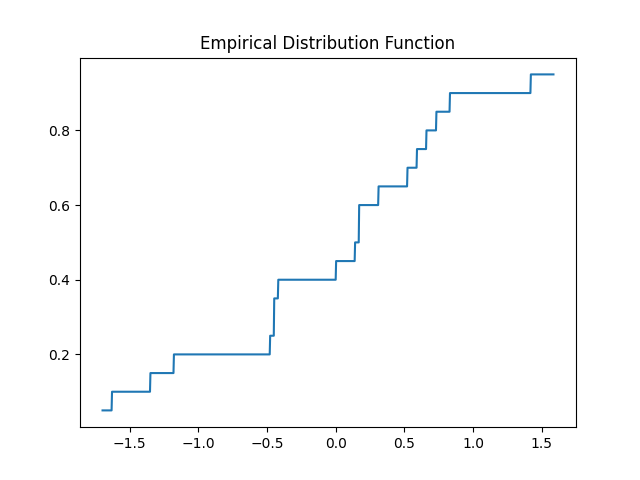
\includegraphics[width=10cm]{dist.png}
    \caption{График функции распределения}
\end{figure}

\begin{figure}[h]
    \centering
    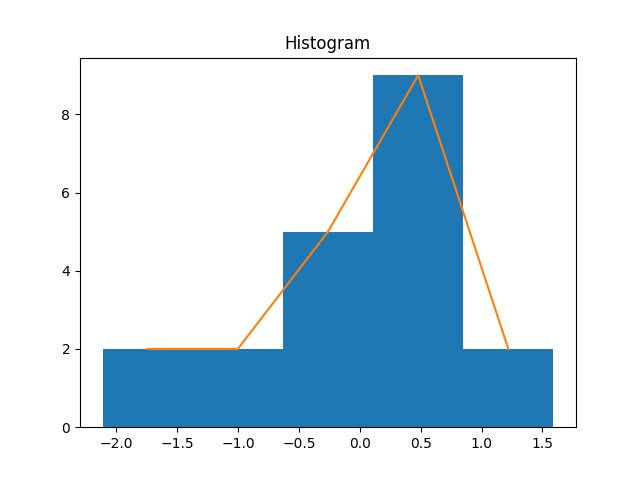
\includegraphics[width=10cm]{hist.png}
    \caption{График гистограммы распределения}
\end{figure}


\end{document}